\section{Planteamiento del Problema}\label{cap:problema}

\subsection{Descripción del problema}

Lush Beauty es un salón de belleza que ofrece servicios de manicura, pedicura, depilación, cejas y pestañas, y un catálogo para niñas denominado \textit{Lush Little Princess}. Hasta la fecha, la administradora —quien además opera como especialista— controlaba los ingresos y la liquidación del personal en un archivo de hojas de cálculo con tres hojas, una por especialista. En cada fila se registran la fecha, el cliente, el servicio, el monto, el descuento, la comisión del 35~\% calculada sobre el precio de lista, la ganancia neta del salón y la propina.


La Tabla~\ref{tab:v4_1} resume la planilla de ejemplo de agosto de 2026, que reproduce el formato y el tipo de datos que recibe el salón; las cifras son ilustrativas y se contrastarán con los registros reales durante la recolección de datos. En ese mes de ejemplo se anotaron 91 servicios con un monto bruto de Bs~11.462, de los cuales se cobraron Bs~10.038 tras aplicar descuentos por Bs~1.424 (12,4~\% del bruto). La comisión total ascendió a Bs~4.011,70 y las propinas a Bs~85. Asimismo, la administradora concentró 57 de los 91 servicios (62,6~\%) y el 80,8~\% del monto bruto, como se aprecia en la Figura~\ref{fig:v4_1}, lo que confirma que la misma persona administra el negocio y presta servicios.


\vspace{8pt}{\footnotesize\setstretch{1.0}
\begin{longtable}{>{\raggedright\arraybackslash}p{0.2722\dimexpr\linewidth-12\tabcolsep\relax}>{\raggedright\arraybackslash}p{0.1183\dimexpr\linewidth-12\tabcolsep\relax}>{\raggedright\arraybackslash}p{0.1361\dimexpr\linewidth-12\tabcolsep\relax}>{\raggedright\arraybackslash}p{0.1420\dimexpr\linewidth-12\tabcolsep\relax}>{\raggedright\arraybackslash}p{0.1893\dimexpr\linewidth-12\tabcolsep\relax}>{\raggedright\arraybackslash}p{0.1420\dimexpr\linewidth-12\tabcolsep\relax}}
\caption{Actividad de la planilla de ejemplo por especialista, agosto de 2026}\label{tab:v4_1}\\
\toprule
\textbf{Especialista} & \textbf{Servicios} & \textbf{Bruto (Bs)} & \textbf{Cobrado (Bs)} & \textbf{Comisión 35~\% (Bs)} & \textbf{Propinas (Bs)} \\
\midrule\endfirsthead
\toprule
\textbf{Especialista} & \textbf{Servicios} & \textbf{Bruto (Bs)} & \textbf{Cobrado (Bs)} & \textbf{Comisión 35~\% (Bs)} & \textbf{Propinas (Bs)} \\
\midrule\endhead
\bottomrule\endfoot
\bottomrule\endlastfoot
Paty & 21 & 1.060 & 939 & 371,00 & 35 \\
Katherine & 13 & 1.142 & 987 & 399,70 & 10 \\
Marisol (administradora) & 57 & 9.260 & 8.112 & 3.241,00 & 40 \\
\textbf{Total} & \textbf{91} & \textbf{11.462} & \textbf{10.038} & \textbf{4.011,70} & \textbf{85} \\
\end{longtable}}
\nota{Elaboración propia a partir de la planilla de pagos de ejemplo (agosto de 2026) que representa los datos que recibe el salón. Cifras ilustrativas. Moneda: bolivianos (Bs).}

\begin{figure}[H]
\caption{Servicios y monto bruto por especialista en la planilla de ejemplo, agosto de 2026}\label{fig:v4_1}
\centering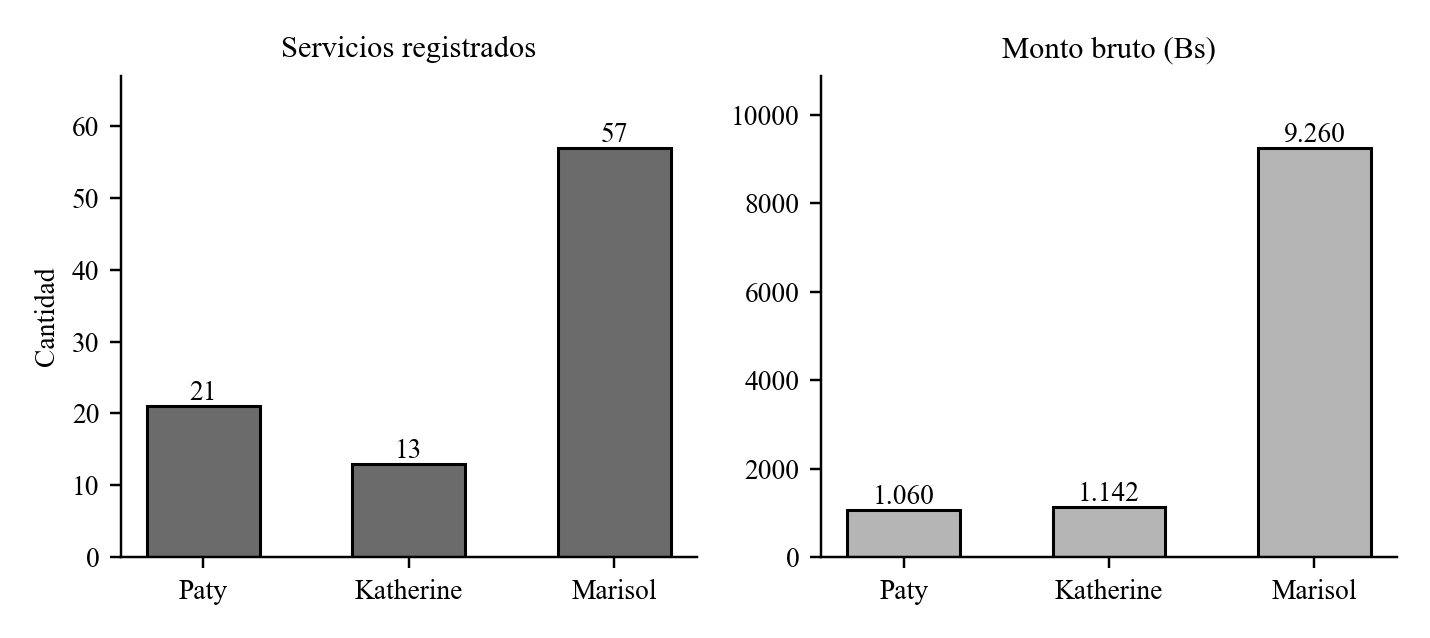
\includegraphics[width=0.9\linewidth]{img/fig_servicios_especialista.png}
\end{figure}
\nota{Elaboración propia a partir de la planilla de pagos de ejemplo (agosto de 2026). Cifras ilustrativas.}

El análisis de la planilla permitió detectar inconsistencias que afectan la confiabilidad de la información (Tabla~\ref{tab:v4_2}). Una de ellas tiene incidencia económica directa: al calcularse la comisión sobre el precio de lista y no sobre el monto cobrado, el salón absorbe íntegramente los descuentos; de haberse aplicado el 35~\% sobre lo cobrado, la comisión total habría sido de Bs~3.513,30, es decir, Bs~498,40 menos. Más allá de la decisión comercial que corresponda, la planilla no permite sostener ni auditar ese criterio.


\vspace{8pt}{\small\setstretch{1.0}
\begin{longtable}{>{\raggedright\arraybackslash}p{0.2195\dimexpr\linewidth-6\tabcolsep\relax}>{\raggedright\arraybackslash}p{0.4269\dimexpr\linewidth-6\tabcolsep\relax}>{\raggedright\arraybackslash}p{0.3536\dimexpr\linewidth-6\tabcolsep\relax}}
\caption{Inconsistencias detectadas en la planilla de ejemplo de agosto de 2026}\label{tab:v4_2}\\
\toprule
\textbf{Hallazgo} & \textbf{Evidencia en la planilla} & \textbf{Consecuencia} \\
\midrule\endfirsthead
\toprule
\textbf{Hallazgo} & \textbf{Evidencia en la planilla} & \textbf{Consecuencia} \\
\midrule\endhead
\bottomrule\endfoot
\bottomrule\endlastfoot
Servicio en texto libre & «PEDI» y « PEDI»; «KAPPING» y «KAPPIN»; «SOFTGEL» y «SOFT GEL» & No es posible totalizar por servicio sin depuración manual \\
Combos sin descomponer & «LIFTING+HENNA+CEJAS»; «MANI+PEDI+TIPS» & El precio no es trazable al catálogo oficial \\
Precios fuera de catálogo & «MANI GEL» cobrado a Bs~112 (catálogo: Bs~120) & Diferencias entre lista y cobro sin motivo registrado \\
Estructura distinta entre hojas & Una hoja sin columna de ganancia neta; propinas en columnas sin nombre; una suma almacenada como texto & Riesgo de errores de suma y de omisión \\
Sin método de pago & No existe la columna & No se puede cuadrar la caja por efectivo, QR o transferencia \\
Sin cancelaciones ni deducciones & No existen columnas para adelantos, faltas o materiales & La liquidación neta queda incompleta \\
Clientes en texto libre & nombres con anotaciones personales (p. ej., relaciones con otras clientas); nombres duplicados con espacios finales & No existe ficha de cliente ni historial \\
\end{longtable}}
\nota{Elaboración propia a partir del análisis de la planilla de pagos de ejemplo (agosto de 2026).}

En consecuencia, el problema se manifiesta en tres planos: la \textbf{exactitud} (riesgo de error en comisiones y totales), la \textbf{eficiencia} (la liquidación semanal exige revisión manual de cada hoja) y la \textbf{trazabilidad} (no se conserva quién modificó un dato ni su valor anterior). A ello se suma la dependencia de una única administradora que registra la información durante la jornada, de pie y, en general, desde el teléfono móvil, una condición para la cual una hoja de cálculo no está diseñada.


\subsection{Delimitación}

\textbf{Espacial:} salón de belleza Lush Beauty, ciudad de Santa Cruz de la Sierra, Bolivia. \textbf{Temporal:} diagnóstico con la planilla de ejemplo de agosto de 2026, línea base retrospectiva y prueba piloto en enero de 2027. \textbf{Poblacional:} la administradora y las especialistas del salón (tres personas) y los registros de servicios generados en el periodo. \textbf{Temática:} gestión de caja y liquidación de comisiones; quedan fuera la agenda de reservas, la facturación electrónica y el inventario.


Adicionalmente, la ampliación hacia el soporte para decisiones establece las siguientes delimitaciones y restricciones:

\begin{vinetas}
\item Ámbito temático: servicios, clientes mínimos, cobros, descuentos, propinas, comisiones, deducciones, cierres, importación, auditoría y reportes.
\item Fuera del MVP: agenda de reservas, facturación electrónica, inventario, reconocimiento visual de uñas, pasarela bancaria automática y aplicación React Native independiente.
\item Restricción metodológica: los datos mensuales representativos no permiten afirmar efectos económicos observados ni justificar modelos predictivos complejos sin historial adicional.
\end{vinetas}

\subsection{Formulación del problema}

\textbf{Pregunta principal:} ¿De qué manera influye la implementación de un sistema web móvil de gestión de caja y nómina en la eficiencia y la exactitud de la liquidación semanal de comisiones del salón Lush Beauty de la ciudad de Santa Cruz de la Sierra durante el periodo noviembre de 2026 – marzo de 2027?


Como ampliación orientada a la toma de decisiones, se formula además la siguiente pregunta complementaria: ¿De qué manera el diseño y uso de un sistema inteligente de soporte para decisiones, basado en registros financieros verificables, simulación de escenarios, comparación multicriterio y recomendaciones explicables, puede contribuir a mejorar la calidad, oportunidad y trazabilidad de las decisiones de caja, precios, descuentos y comisiones del salón Lush Beauty, sin perder eficiencia operativa?

\subsection{Sistematización del problema}

\begin{vinetas}
\item ¿Cómo se realizan actualmente el registro de servicios, el cobro y la liquidación de comisiones en el salón?
\item ¿Qué inconsistencias y riesgos presenta la planilla actual y qué impacto económico tienen?
\item ¿Qué funcionalidades ofrecen los sistemas comerciales similares y qué brechas dejan frente a las necesidades del salón?
\item ¿Qué requisitos, reglas de negocio y arquitectura debe tener un sistema que resuelva estas brechas?
\item ¿En qué medida el sistema reduce el tiempo de liquidación y los errores de cálculo, y qué usabilidad perciben sus usuarias?
\item ¿Qué decisiones financieras y operativas del salón (descuentos, precios, comisiones y cierres de caja) puede apoyar un sistema de soporte basado en simulación de escenarios y comparación multicriterio?
\item ¿Cómo se garantiza que las recomendaciones del sistema sean explicables, trazables y estén siempre sujetas a la aprobación humana?
\end{vinetas}
